\documentclass[]{article}

\usepackage{amsmath}  % AMS math package
\usepackage{amssymb}  % AMS symbol package
\usepackage{bm}       % bold math
\usepackage{graphicx} % Include figure files
\usepackage{dcolumn}  % Align table columns on decimal point
\usepackage{multirow} % Multirow/column tables
\usepackage{hyperref} % Hyperlinks
\usepackage{caption}
\usepackage{listings}
%\usepackage{subcaption}

\newcommand{\unit}[2]{#1~\mathrm{#2}}

\begin{document}

\title{Molecular Dynamics}
\author{Justin Browne}
\date{}
\maketitle

\begin{abstract}
This work covers the development and application of a molecular dynamics simulation of Argon.
The Argon gas is modeled with the 6-12 Lennard-Jones potential.
The data from the simulation were compared to experimental pressure and diffusion coefficient data.
\end{abstract}

\section{Introduction}
The Lennard-Jones potetial is a potential commonly used to model the interaction between two atoms or molecules \cite{jones1924}.
The potential takes the form
\[
\phantom{.} V_{LJ} = \left(\frac{\lambda_{n}}{r}\right)^{n} - \left(\frac{\lambda_{m}}{r}\right)^{m} .
\]
One of the most common forms of this potential is the "6-12 potential," which is given by
\[
\phantom{.} V_{LJ} = 4\varepsilon \left[ \left(\frac{\sigma}{r}\right)^{12} - \left(\frac{\sigma}{r}\right)^{6} \right] ,
\]
is shown in Figure~\ref{fig:LJpot}.

\begin{figure}[htb]
	\centering
	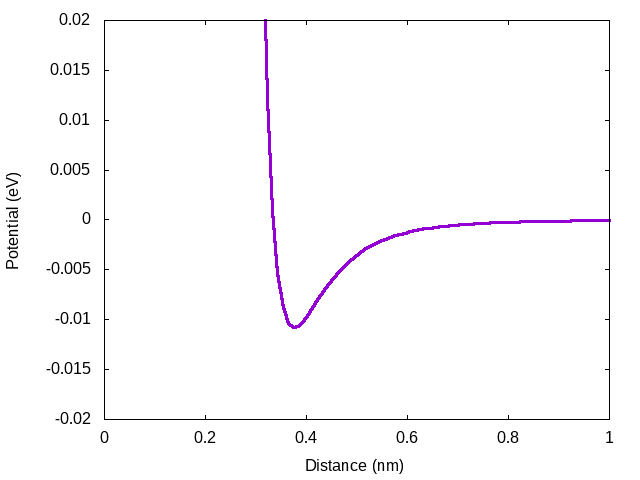
\includegraphics[width=\textwidth]{figures/LJpot.png}
	\caption{The "6-12 Lennard-Jones Potential" for an Argon gas.}
	\label{fig:LJpot}
\end{figure}

\section{Implementation}
The time integration was performed using the velcity verlet algorithm, which is given by
\begin{align*}
\vec{v}(t + \tfrac{1}{2} dt) & = \vec{v}(t)                   + \tfrac{1}{2} \vec{a}(t) dt      \\
\vec{r}(t + dt)              & = \vec{x}(t)                   + \vec{v}(t + \tfrac{1}{2} dt) dt \\
\vec{v}(t + dt)              & = \vec{v}(t + \tfrac{1}{2} dt) + \tfrac{1}{2} \vec{a}(t + dt) .
\end{align*}
The advantages of the velocity Verlet algorithm over the standard verlet aglorigthm are:
1. superior numerical precision, and
2. the velocity and position at the end of the time step are directly computed from the velocity and position at the start of the time step \cite{swope1982}.

\subsection{Thermostat}
A simple thermostat was implemented to adjust the temperature of the system by scaling the velocity of all of the particles in the system.
Using the following relations
\begin{align*}
T &\propto K \\
K &= \frac{1}{2} m v^{2} \\
\frac{T_{1}}{T_{2}} &= \frac{v_{1}^{2}}{v_{2}^{2}} ,
\end{align*}
the velocities were scaled by a factor of $\sqrt{\frac{T_{\mathrm{target}}}{T_{\mathrm{current}}}}$.
The thermostat can be turned on and off at specified times.

\subsection{Verification}
To verify the simulation, a simple two-particle system was implemented.
The expected behavior of the system would be similar to a harmonic oscillator, since the potential is similar near the minimum of the potential.
Thus, we would expect the distance between the two particles to increase and decrease approximately sinusoidally, with a constant period and amplitude.

\begin{lstlisting}[mathescape]
for each particle:
	calculate v(t+$\tfrac{1}{2}$dt)
	calculate r(t+dt)
	calculate a(t+dt)
	calculate v(t+dt)
\end{lstlisting}

\begin{figure}[htb]
	\centering
	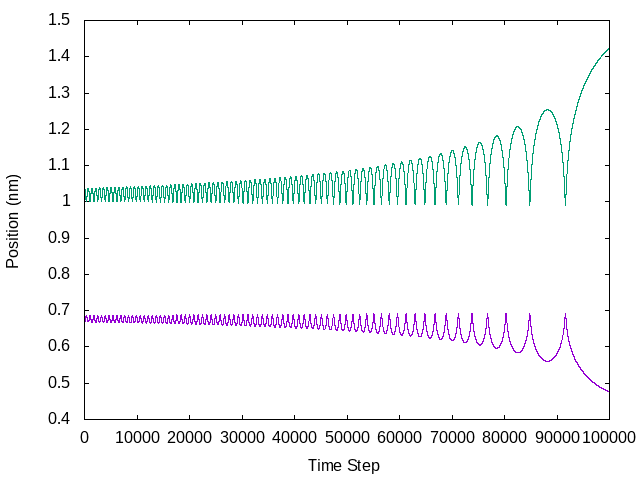
\includegraphics[width=\textwidth]{figures/temp_growth.png}
	\caption{The positions of two particles interacting via the "6-12 Lennard-Jones Potential" using the computational algorithm with one loop.}
	\label{fig:temp_growth}
\end{figure}

Figure~\ref{fig:temp_growth} shows the results of this method, and it can be seen that the results do not match the expectations.
The amplitude and period increase over time; this behavior violates the conservation of energy.
This can be seen in other situations through an increase in energy after the thermostat turns off.
The reason for this is the algorithm above.
The acceleration is not calculated using the correct positions; the positions must all be updated before the acceleration for any particle is calculated, as in the algorithm below.
Figure~\ref{fig:no_growth} shows the results of using that algorithm, and it agrees with our expectations.
Other simulations now do not experience the temperature increase.

\begin{lstlisting}[mathescape]
for each particle:
	calculate v(t+$\tfrac{1}{2}$dt)
	calculate r(t+dt)
for each particle:
	calculate a(t+dt)
for each particle:
	calculate v(t+dt)
\end{lstlisting}

\begin{figure}[htb]
	\centering
	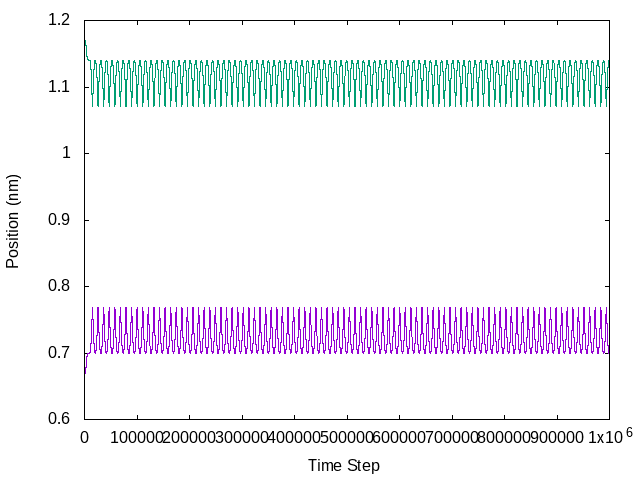
\includegraphics[width=\textwidth]{figures/no_growth.png}
	\caption{The positions of two particles interacting via the "6-12 Lennard-Jones Potential" using the computational algorithm with multiple loops.}
	\label{fig:no_growth}
\end{figure}

Another test to verify the simulation is to check that the conservation of energy holds.
Figure~\ref{fig:energy_cons} shows the total energy of the system.
It shows that there is some variation in the total energy, but even after the thermostat is turned off, there does not seem to be any long term trend in an energy change.

\begin{figure}[htb]
	\centering
	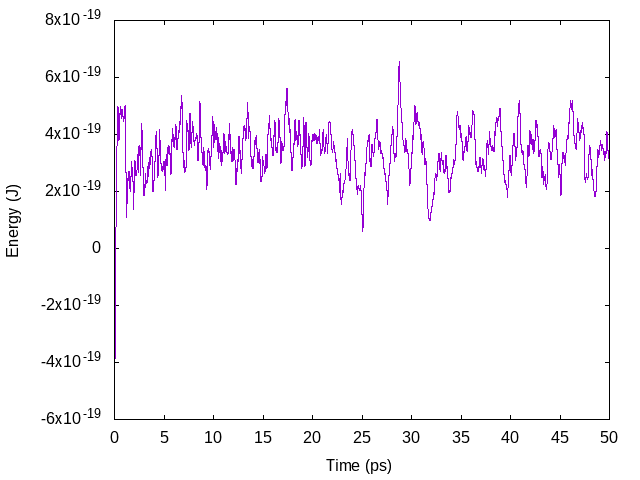
\includegraphics[width=\textwidth]{figures/energy_cons.png}
	\caption{The total energy of a simulation at $T = \unit{300}{K}$. The thermostat runs from iteration 1000 to 20000.}
	\label{fig:energy_cons}
\end{figure}

\section{Simulation Results}
All of the following simulations used the following parameters, unless otherwise specified.
The time between iterations was $\unit{10^{-15}}{s}$, with a total of 50000 iterations.
The thermostat was run every 100 iterations, starting at iteration 1000 and ending at iteration 20000.
The starting configuration was a 3x3x3 FCC lattice, meaning the simulation contained 108 particles.
The starting temperature was varied between $\unit{300}{K}$ and $\unit{350}{K}$.

\subsection{Pressure}
The pressure is calculated using the following equation from \cite{cheung1977}
\[
P = \rho k_{B} T - \frac{1}{DV} \left< \sum_{i,j} \vec{r_{ij}} \cdot \vec{F_{ij}} \right> .
\]
The ideal gas law $P V = N k_{B} T$, meaning $P = A T$, where $A = k_{B} \rho$.
Using the parameters of the simulations, $A = \unit{2.87 \times 10^{5}}{Pa/K}$.
The linear fit of the data from the simulations is shown in figure~\ref{fig:P_T}, and is given by $P = p_{0} + p_{1} T$, where $p_{0} = \unit{(0.14 \pm 1.18) \times 10^{6}}{Pa}$ and $p_{1} = \unit{(2.87 \pm 0.04)\times 10^{5}}{Pa/K}$.
Thus the simulations reproduces the expected behavior of the system's pressure with respect to temperature.

\begin{figure}[htb]
	\centering
	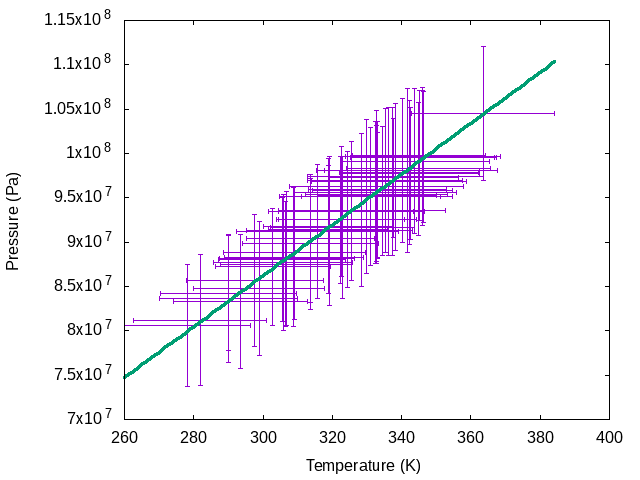
\includegraphics[width=\textwidth]{figures/P_T.png}
	\caption{The pressure as it varies with temperature and a linear fit.}
	\label{fig:P_T}
\end{figure}

\subsection{Diffusion Coefficient}
The diffusion coefficient describes the rate at which particles spread out from their starting positions.
\[
	D(t) = \frac{1}{6 N t} \sum_{n=1}^{N}\left( r_{j}(t) - r_{j}(0)\right)^{2}
\]
was used to compute the diffusion constant \cite{weizhong2008}.
Using the relation
\[
	D \propto \frac{T^{3/2}}{P}
\]
and data from \cite{kestin1984}, we can compare the diffusion coefficient from the simulations to real world data.
The results are shown in figure~\ref{fig:D_T}.
One can see that the diffusion coefficient calculated from the simulations do not match the data.
The problem, however, may not lie with the simulation, but instead with the calculation of the diffusion coefficient.
Because of the periodic boundaries of the simulation, the calculated displacement of a particle might be incorrect.
Since the particles are constrained to a finite volume, one would expect the calculated value to be an underestimate of the true value, which is the behavior shown in these data.

\begin{figure}[htb]
	\centering
	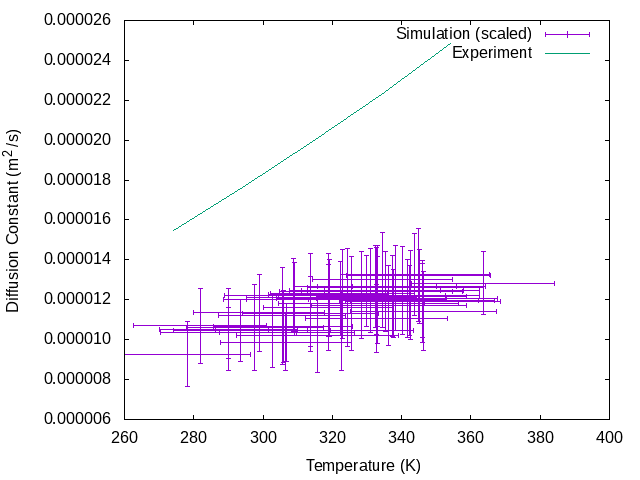
\includegraphics[width=\textwidth]{figures/D_T.png}
	\caption{The diffusion coefficient as it varies with temperature, from the simulation (scaled to correspond to $\unit{1.031}{bar}$) and from \cite{kestin1984}.}
	\label{fig:D_T}
\end{figure}

\section{Further Study}
More sophisticated thermostats could be implemented.
These could provide more accurate models of interactions with a heat bath.

The calculation of the diffusion coefficient could be improved by keeping track of the position of the particle, without accounting for the periodic boundary condition, but account for it during the force calculation.
This would, hopefully, provide better agreement of the diffusion coefficient with experiment.

\begin{thebibliography}{}
	\bibitem{jones1924}
		J. E. Jones, Proc. R. Soc. Lond. A, 106, 463--477 (1924)
	\bibitem{swope1982}
		Swope, W.~C., et al., J. Chem. Phys, 76, 637--649 (1982)
	\bibitem{cheung1977}
		Cheung, P., Molecular Physics, 33, 519--526 (1977)
	\bibitem{weizhong2008}
		Wei-Zhong, L., Cong, C. \& Jian, Y. Heat Trans. Asian Res. 37, 86--93 (2008)
	\bibitem{kestin1984}
		Kestin, J., et al. Journal of Physical and Chemical Reference Data 13, 229--303 (1984)
\end{thebibliography}

\end{document}
